\section{Ejercicio 5}

\subsection{Entrada flotante}
En está subsección vamos a desarrollar el comportamiento que tiene las compuestas TTL y CMOS, por medio de los siguientes circuitos:

\begin{figure}[H]
	\centering
	\begin{minipage}{0.4\textwidth}
    		\centering
		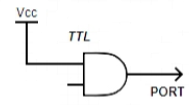
\includegraphics[width=0.25\textwidth]{Ejercicio5/TTL.png}
		\caption{Circuito para TTL AND}
	\end{minipage}
	\hspace{5mm}
	\begin{minipage}{0.4\textwidth}
		\centering
		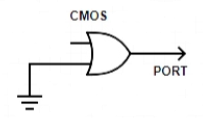
\includegraphics[width=0.25\textwidth]{Ejercicio5/CMOS.png}
		\caption{Circuito para CMOS OR}
	\end{minipage}
\end{figure}
El resultado obtenido fue:
\begin{figure}[H]
	\centering
	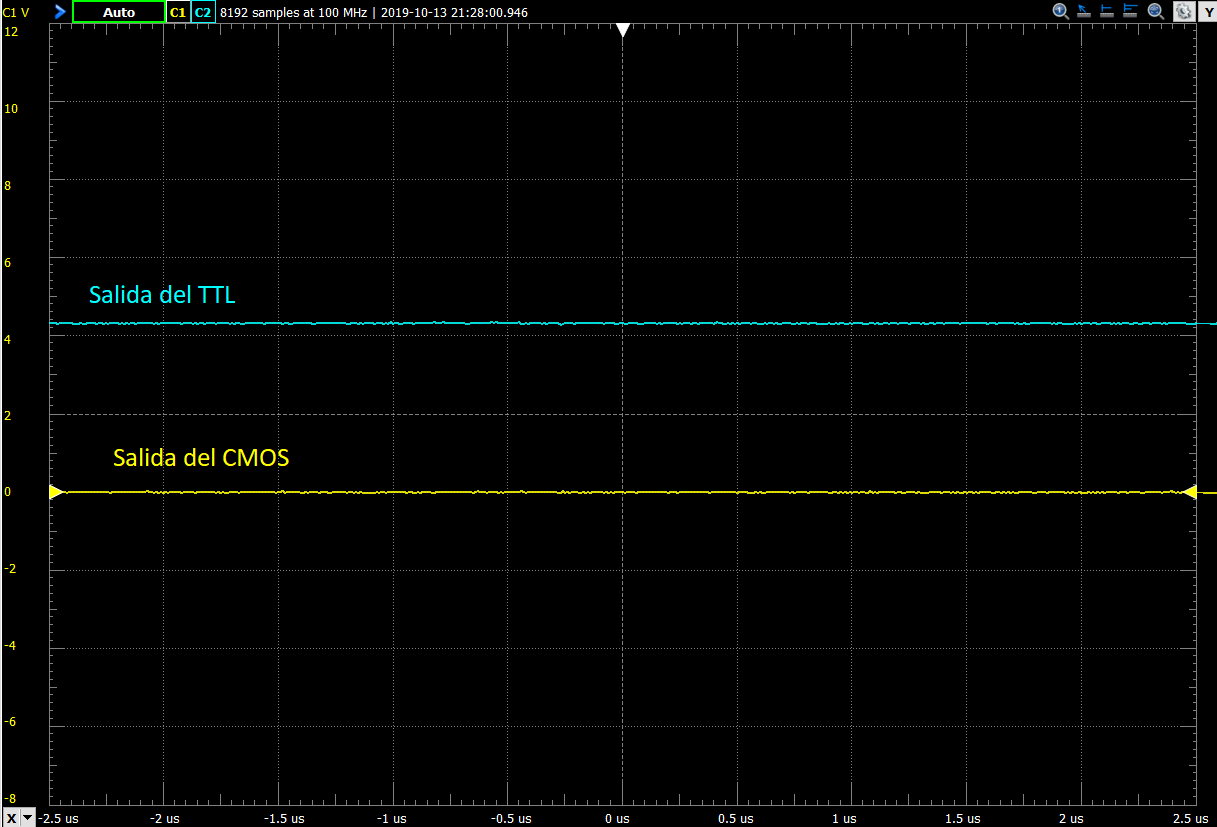
\includegraphics[width=0.3\textwidth]{Ejercicio5/Flotante.png}
	\caption{Resultados de los circuitos}
\end{figure}

En conclusión, la entrada flotante del circuito TTL produjo una salida alta. Esto significa que por default tenemos una entrada alta en el mismo y esto se debe a que, los circuitos de la familia LS utilizan la tecnología TTL donde poseen un pull up interno de forma tal que, al no enviar entrada, el transistor se encuentra igualmente polarizado y como consecuencia es como si recibiera una entrada high. Esto se debe a que es necesario que el ruido tenga una amplitud considerablemente grande para poder activar la compuerta.\\
Mientras que en el caso del circuito CMOS, obtenemos que la salida oscila a una frecuencia de 50 Hz. Esto se debe a que el transistor CMOS presenta una alta impedancia de entrada, lo que vuelve cualquier entrada flotante susceptible al ruido y este es lo suficientemente fuerte como para entrar en la zona lineal de operación de esta.

\subsection{Compatibilidad entre TTL y CMOS}
A continuación vamos a ver los problemas presentados en el circuito de la figura \ref{fig:eje5_1}, así como los problemas que está presenta.

\begin{figure}[H]
	\centering
	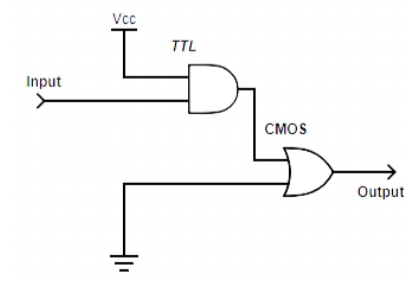
\includegraphics[width=0.3\textwidth]{Ejercicio5/TTL_CMOS.png}
	\caption{TTL cargando CMOS}
	\label{fig:eje5_1}
\end{figure}

Teniendo en cuenta los datos siguientes:

\begin{table}[H]
	\centering
	\begin{tabular}{|c|c|c|c|c|}
		\hline
		Tecnología & $V_{IL_{max}}$	& $V_{IH_{min}}$ & $V_{OL_{max}}$ & $V_{OH_{min}}$\\
		\hline
		{74LS08} & 0.8 V & 2 V & 0.5 V & 2.7 V\\
		\hline
		{74HC32} & 1.35 V & 3.15 V & 0.26 V & 3.98 V\\
		\hline
	\end{tabular}
\end{table}

Tenemos que el $V_{OH_{min}}$ del TTL es inferior al $V_{IH_{min}}$ del CMOS. Esto causa que, aunque el AND se encuentre en estado alto mientras esté sea menor a 3.15 V, la compuerta OR no va a considerarla como tal dando nos una respuesta diferente a la esperada.
Este tipo de problemas pueden ser solucionados por un level shifter o por un pull up, debido a que el pull up solo va a generar una reducción en el rise time del mismo gracias a que inyecta más corriente, utilizaremos un level shifter para solucionarlo.
Una manera sencilla de aplicar un level shifter puede verse en la figura \ref{fig:eje5_2}.

\begin{figure}[H]
	\centering
	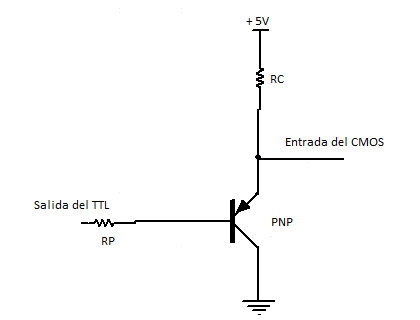
\includegraphics[width=0.3\textwidth]{Ejercicio5/Levelshifter.png}
	\caption{TTL cargando CMOS}
	\label{fig:eje5_2}
\end{figure}

El problema se encuentra solucionado dado que ahora al OR CMOS le va a llegar un $V_{OL_{max}}=2.7+0.7=3.4$ aproximadamente, esto es mayor a 3.15 V solucionando completamente el problema encontrado.

\begin{figure}[H]
	\centering
	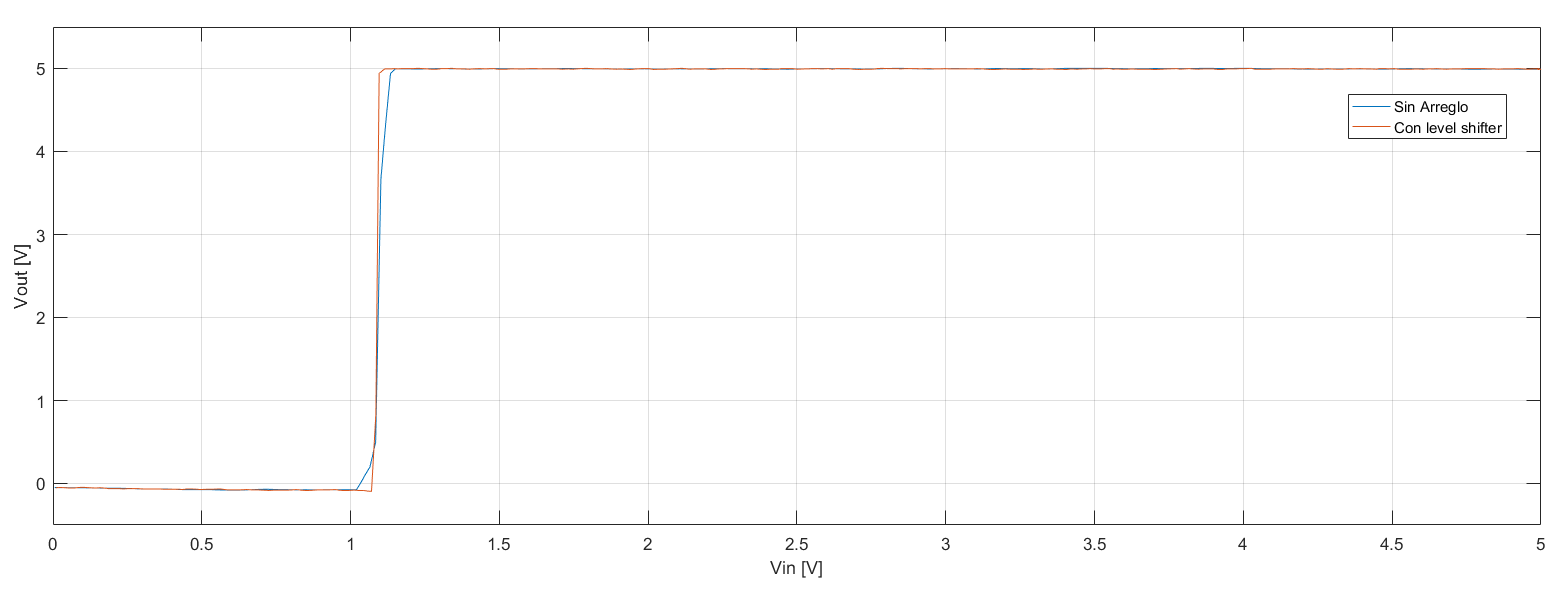
\includegraphics[width=0.3\textwidth]{Ejercicio5/Comparacion.png}
	\caption{Comparación entre sin solución y con solución}
\end{figure}

Podemos concluir, que a pesar de haber aumentado el $V_{IL_{max}}$ y $V_{OL_{max}}$ logramos disminuir los $V_{IH_{min}}$ y $V_{OH_{min}}$. Además, una mayor pendiente lo que significa que el cambio producido por la entrada actúa más rápido que sin haber aplicado la solución, en el sentido de que menores cambios de tensión en la entrada producen mayores cambios en la salida.